\chapter[Paleoclimate and historical climatic niches]{Paleoclimate, Historical Climatic Niches, and Distributional Reconstruction}

\begin{objetivos}
By the end of this chapter, readers should be able to explain how paleoclimatic data are used in SDM; recognize the mid-Holocene, Last Glacial Maximum, and Last Interglacial; harmonize paleoclimatic predictors with baseline model inputs; project models for \textit{Dinizia excelsa} to past climates; evaluate historical climatic stability; identify candidate areas of long-term suitability; and interpret paleoclimate projections as biogeographic hypotheses rather than direct evidence of past occurrence.
\end{objetivos}

\section{Introduction}

The contemporary distribution of an Amazonian tree species reflects both present-day ecological processes and a deeper climatic history. Past changes in temperature, precipitation, seasonality, forest connectivity, and environmental stability may have influenced population persistence, expansion, contraction, and spatial genetic structure.

In SDM, models calibrated with contemporary data can be transferred to reconstructed climates such as the mid-Holocene, Last Glacial Maximum, and Last Interglacial. These projections support hypotheses about climatic stability, potential refugia, historical connectivity, and niche conservatism. Their interpretation requires the same transferability safeguards used for future projections, together with recognition that uncertainties increase backward through climate reconstruction, model choice, and ecological assumptions.

\begin{conceito}[title={\faBook\quad Historical climatic niche}]
A historical climatic-niche projection represents past environmental conditions that a contemporary fitted model classifies as compatible with the species' estimated climatic association. It does not reconstruct the complete historical niche, demonstrate occupancy, or establish population continuity.
\end{conceito}

\section{A climatic timeline from the past to possible futures}

Paleoclimate modeling reconstructs potential distributions under past environmental conditions, whereas future projections explore responses under alternative climate trajectories. Together, these approaches connect historical biogeography, climatic stability, candidate refugia, and future vulnerability.

Here, the modeled climatic association of \textit{Dinizia excelsa} is interpreted along a timeline comprising widely used paleoclimatic periods, baseline conditions, and future GCM scenarios. The comparison asks whether currently suitable areas may also have been suitable in the past and whether they remain suitable under specified future conditions.

\begin{center}
\fbox{
\begin{minipage}{0.90\textwidth}
\centering
\textbf{Climatic timeline used to interpret model projections}

\vspace{0.4cm}

\small
\setlength{\tabcolsep}{4pt}
\begin{tabular}{p{0.12\textwidth}p{0.25\textwidth}p{0.45\textwidth}}
\toprule
\textbf{Time} & \textbf{Period/scenario} & \textbf{Ecological interpretation} \\
\midrule
about 130 ka & Last Interglacial (LIG) & A warm interval before the last glacial cycle, useful for exploring model responses under a climate distinct from the present. \\
about 21 ka & Last Glacial Maximum (LGM) & The coldest phase of the last glacial cycle, associated with major changes in tropical climates and vegetation. \\
about 6 ka & Mid-Holocene & A postglacial interval used to examine relatively recent climatic reorganization and stability. \\
baseline & Contemporary reference & The climatic reference period associated with model calibration or baseline interpretation. \\
2050 & SSP1--2.6 and SSP5--8.5 & Mid-century projections under contrasting forcing pathways. \\
2070 & SSP1--2.6 and SSP5--8.5 & Later-century projections under contrasting forcing pathways. \\
\bottomrule
\end{tabular}
\end{minipage}
}
\end{center}

This timeline is a conceptual framework for comparing stability, loss, gain, and displacement of climatically suitable areas across time slices. Persistent modeled suitability can identify candidates for climatic stability, but a biogeographic refugium requires corroboration from independent evidence such as fossils, phylogeography, population genetics, paleoecology, or historical demography. Areas suitable only in one period should be interpreted especially cautiously when environmental novelty is high.

\begin{conceito}[title={\faBook\quad Temporal SDM}]
Integrating paleoclimate, baseline climate, and future scenarios turns SDM into a comparative temporal framework. The question expands from where a species may find suitable conditions today to how modeled suitability, exposure, and potential persistence vary across time.
\end{conceito}

\section{Relevant paleoclimatic periods}

This chapter considers three principal time slices:

\begin{itemize}
\item the mid-Holocene, approximately 6 thousand years before present;
\item the Last Glacial Maximum, approximately 21 thousand years before present;
\item the Last Interglacial, commonly represented by a time slice around 120--130 thousand years before present, depending on the climate product.
\end{itemize}

These periods represent distinct states of the Earth system and allow us to ask whether areas currently suitable for \textit{Dinizia excelsa} were also classified as climatically suitable under reconstructed past conditions. Exact ages and temporal averaging must follow the metadata of the selected paleoclimate dataset.

\begin{atencao}[title={\faExclamationTriangle\quad Paleoclimate projections are hypotheses}]
Paleoclimate SDMs do not demonstrate that a species occurred in a projected cell. They identify locations that may have been climatically suitable under assumptions of model transferability, partial niche conservatism, adequate paleoclimate reconstruction, and absence of unmodeled dispersal or biotic constraints.
\end{atencao}

\section{Preparing paleoclimatic layers}

Paleoclimatic layers must be harmonized with the predictors used for model calibration. This includes variable definitions, units, temporal summaries, names, resolution, extent, coordinate reference system, grid origin, and spatial mask. When past and baseline layers originate from different products, apparent differences may reflect product bias as well as climate change. Whenever possible, use internally consistent products and compare multiple paleoclimate GCMs.

\rscriptfile{scripts/unidade15/01_estrutura_pastas.R}

\rscriptfile{scripts/unidade15/02_preparar_variaveis_paleoclimaticas.R}

\section{Projecting models to past climates}

Models fitted under baseline conditions are transferred to each paleoclimatic time slice. The exercise assumes that the fitted climatic response is sufficiently conserved for temporal transfer. Extrapolation diagnostics should accompany each projection because past environments may contain values or combinations absent from the calibration domain.

\rscriptfile{scripts/unidade15/03_projetar_modelos_passado.R}

\begin{figure}[H]
\centering
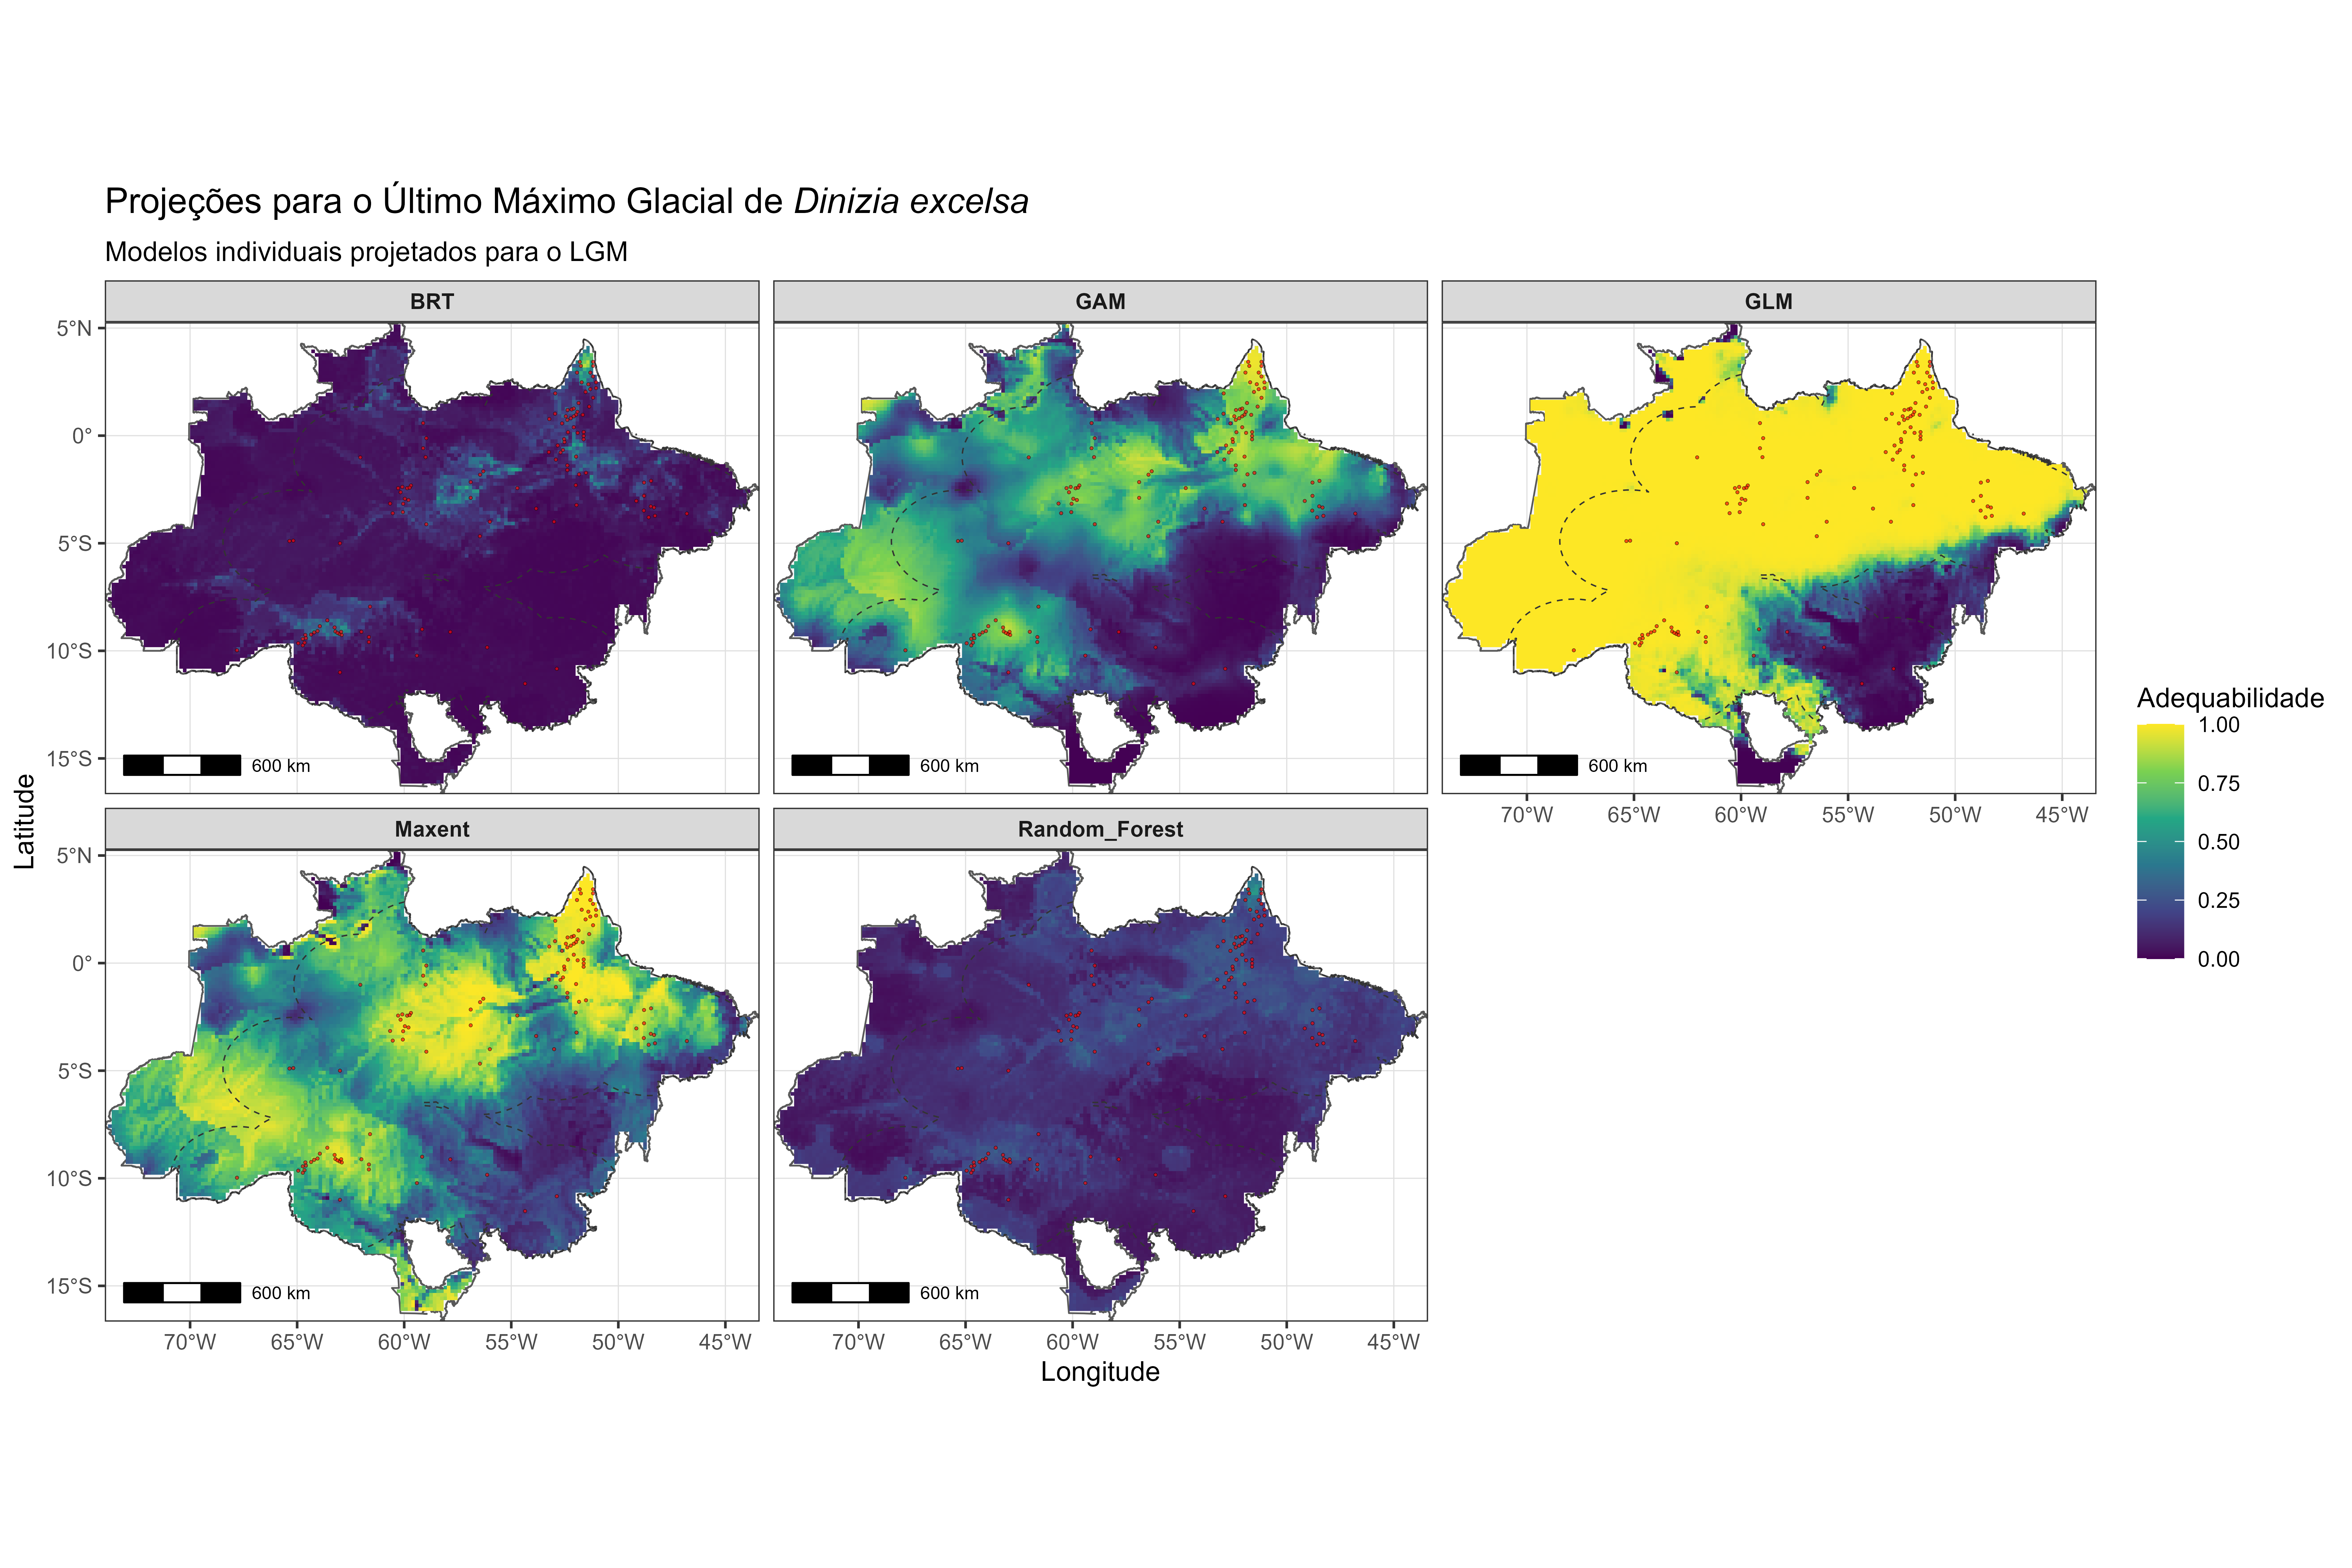
\includegraphics[width=0.98\textwidth]{figuras/unidade15/unidade15_modelos_passado_lgm.png}
\caption{Individual-model projections for \textit{Dinizia excelsa} during the Last Glacial Maximum.}
\label{fig:unidade15_modelos_lgm}
\end{figure}

\section{Paleoclimate ensembles}

Individual projections are combined into an ensemble for each paleoclimatic period. Agreement among algorithms may increase confidence conditional on their shared inputs, but it does not address uncertainty among paleoclimate GCMs or correct common calibration bias. Algorithmic and climatic-model variation should therefore be summarized separately whenever multiple climate reconstructions are available.

\rscriptfile{scripts/unidade15/04_ensemble_passado.R}

\begin{figure}[H]
\centering
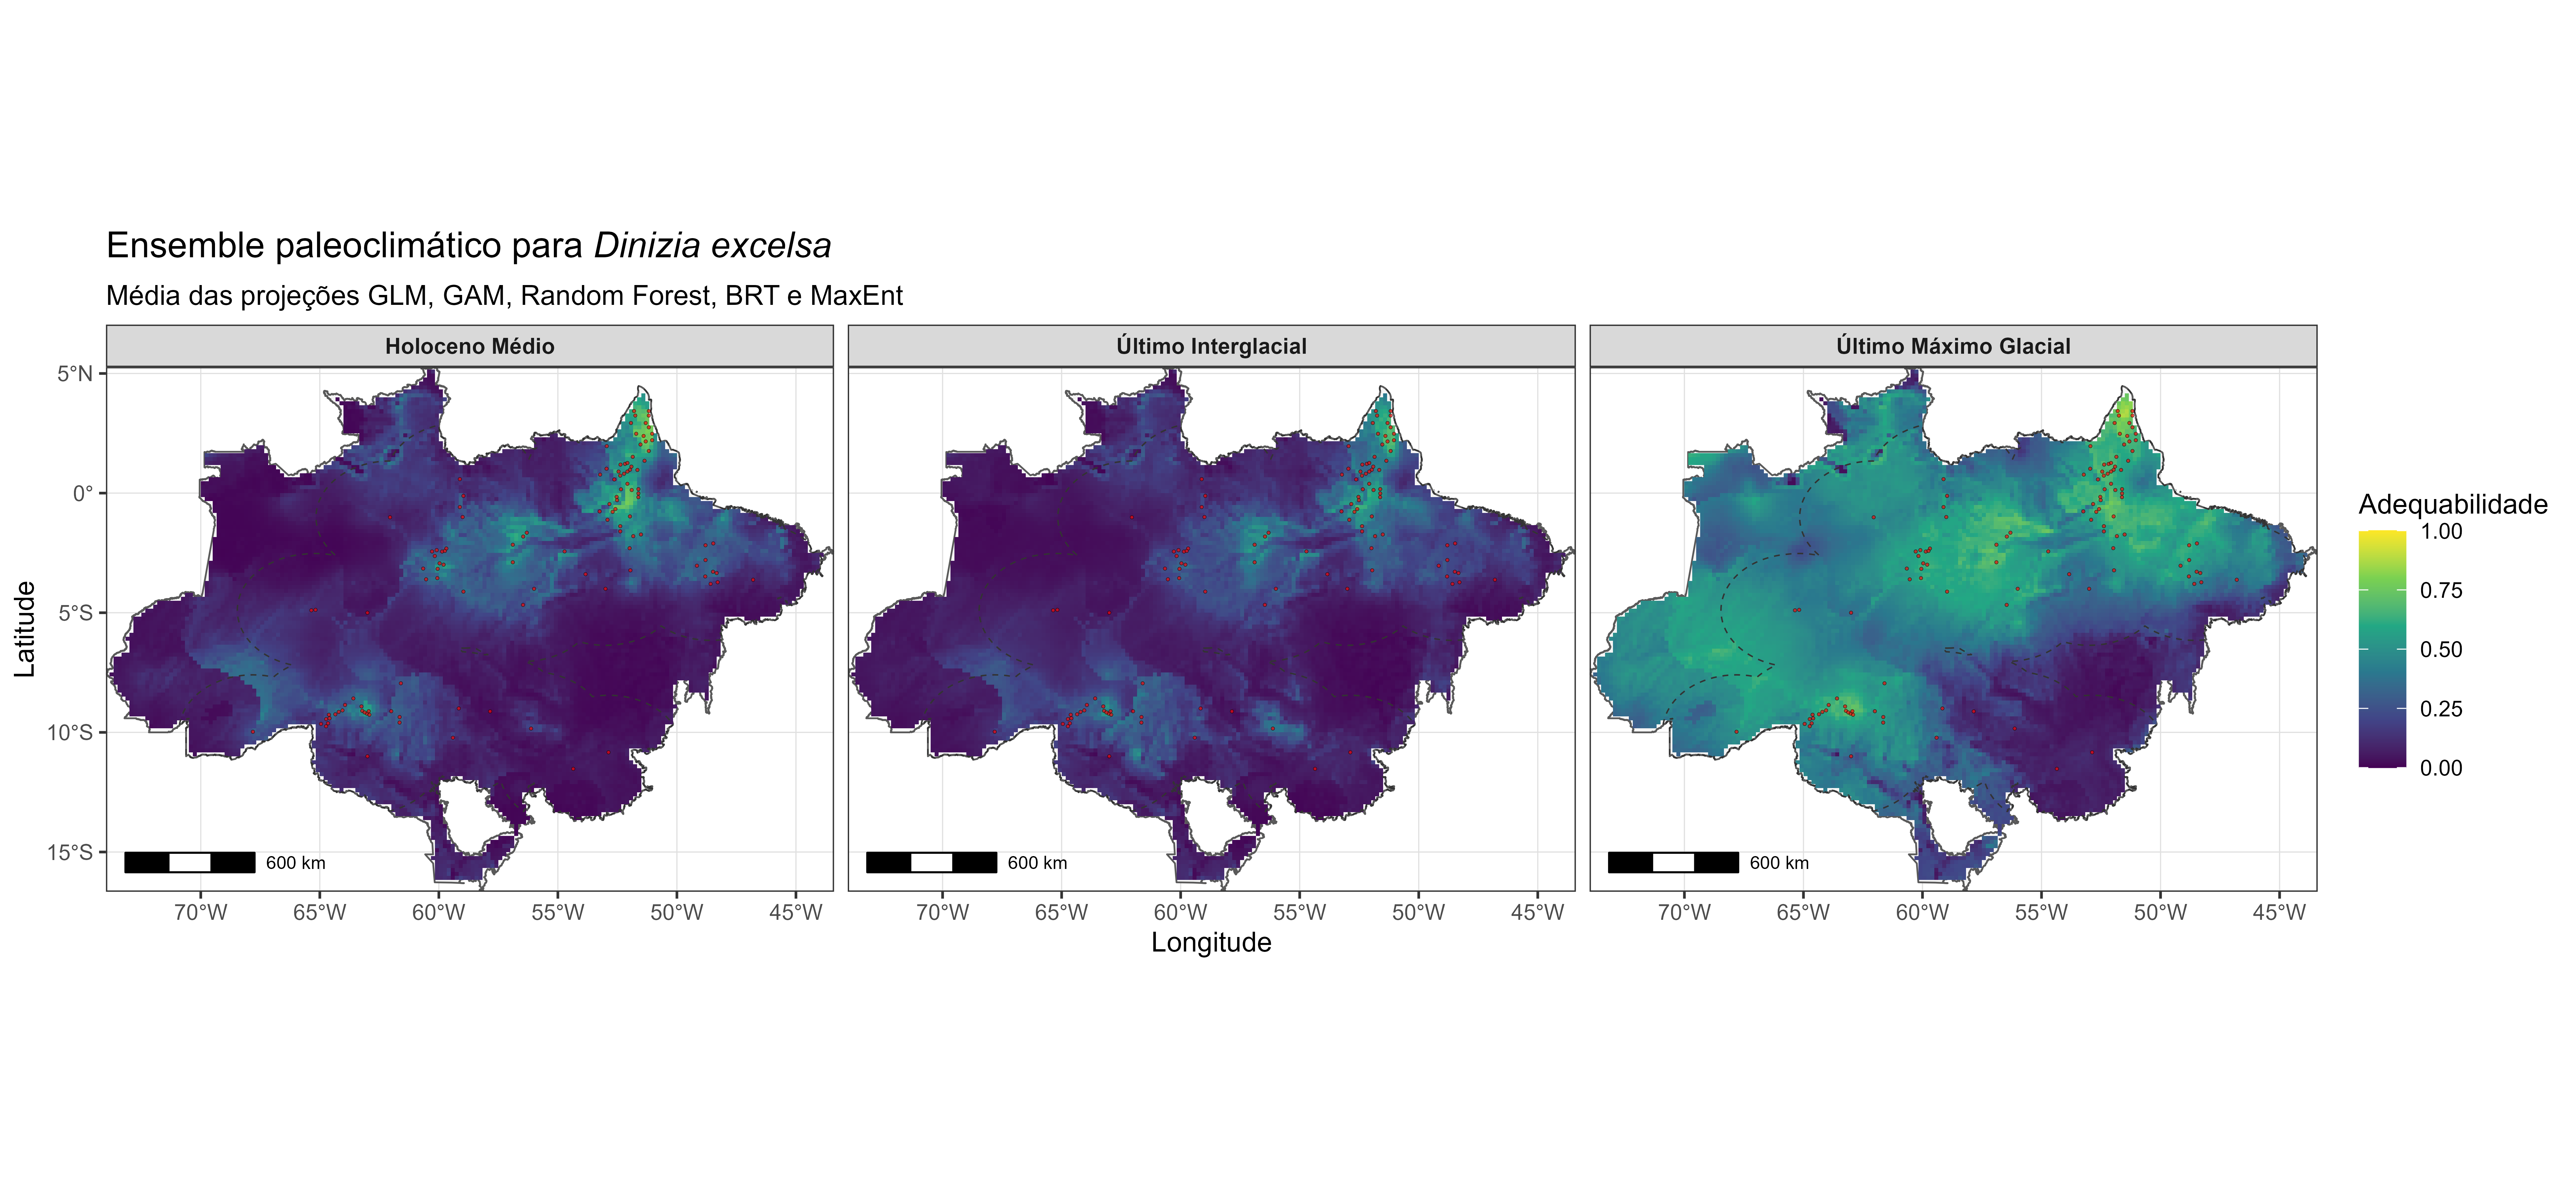
\includegraphics[width=0.96\textwidth]{figuras/unidade15/unidade15_ensemble_passado_periodos.png}
\caption{Paleoclimate ensemble projections of environmental suitability for \textit{Dinizia excelsa}.}
\label{fig:unidade15_ensemble_passado}
\end{figure}

\section{Trajectory through climatic space}

A climatic trajectory compares the contemporary calibration domain with the environmental space available in past periods. Here, an environmental principal component analysis provides a low-dimensional representation of climatic change. The PCA must be fitted to an explicitly defined reference domain and then used to transform other periods with the same centering, scaling, and loadings; fitting a separate PCA to each period would make their axes noncomparable.

\rscriptfile{scripts/unidade15/05_trajetoria_nicho_climatico.R}

\begin{figure}[H]
\centering
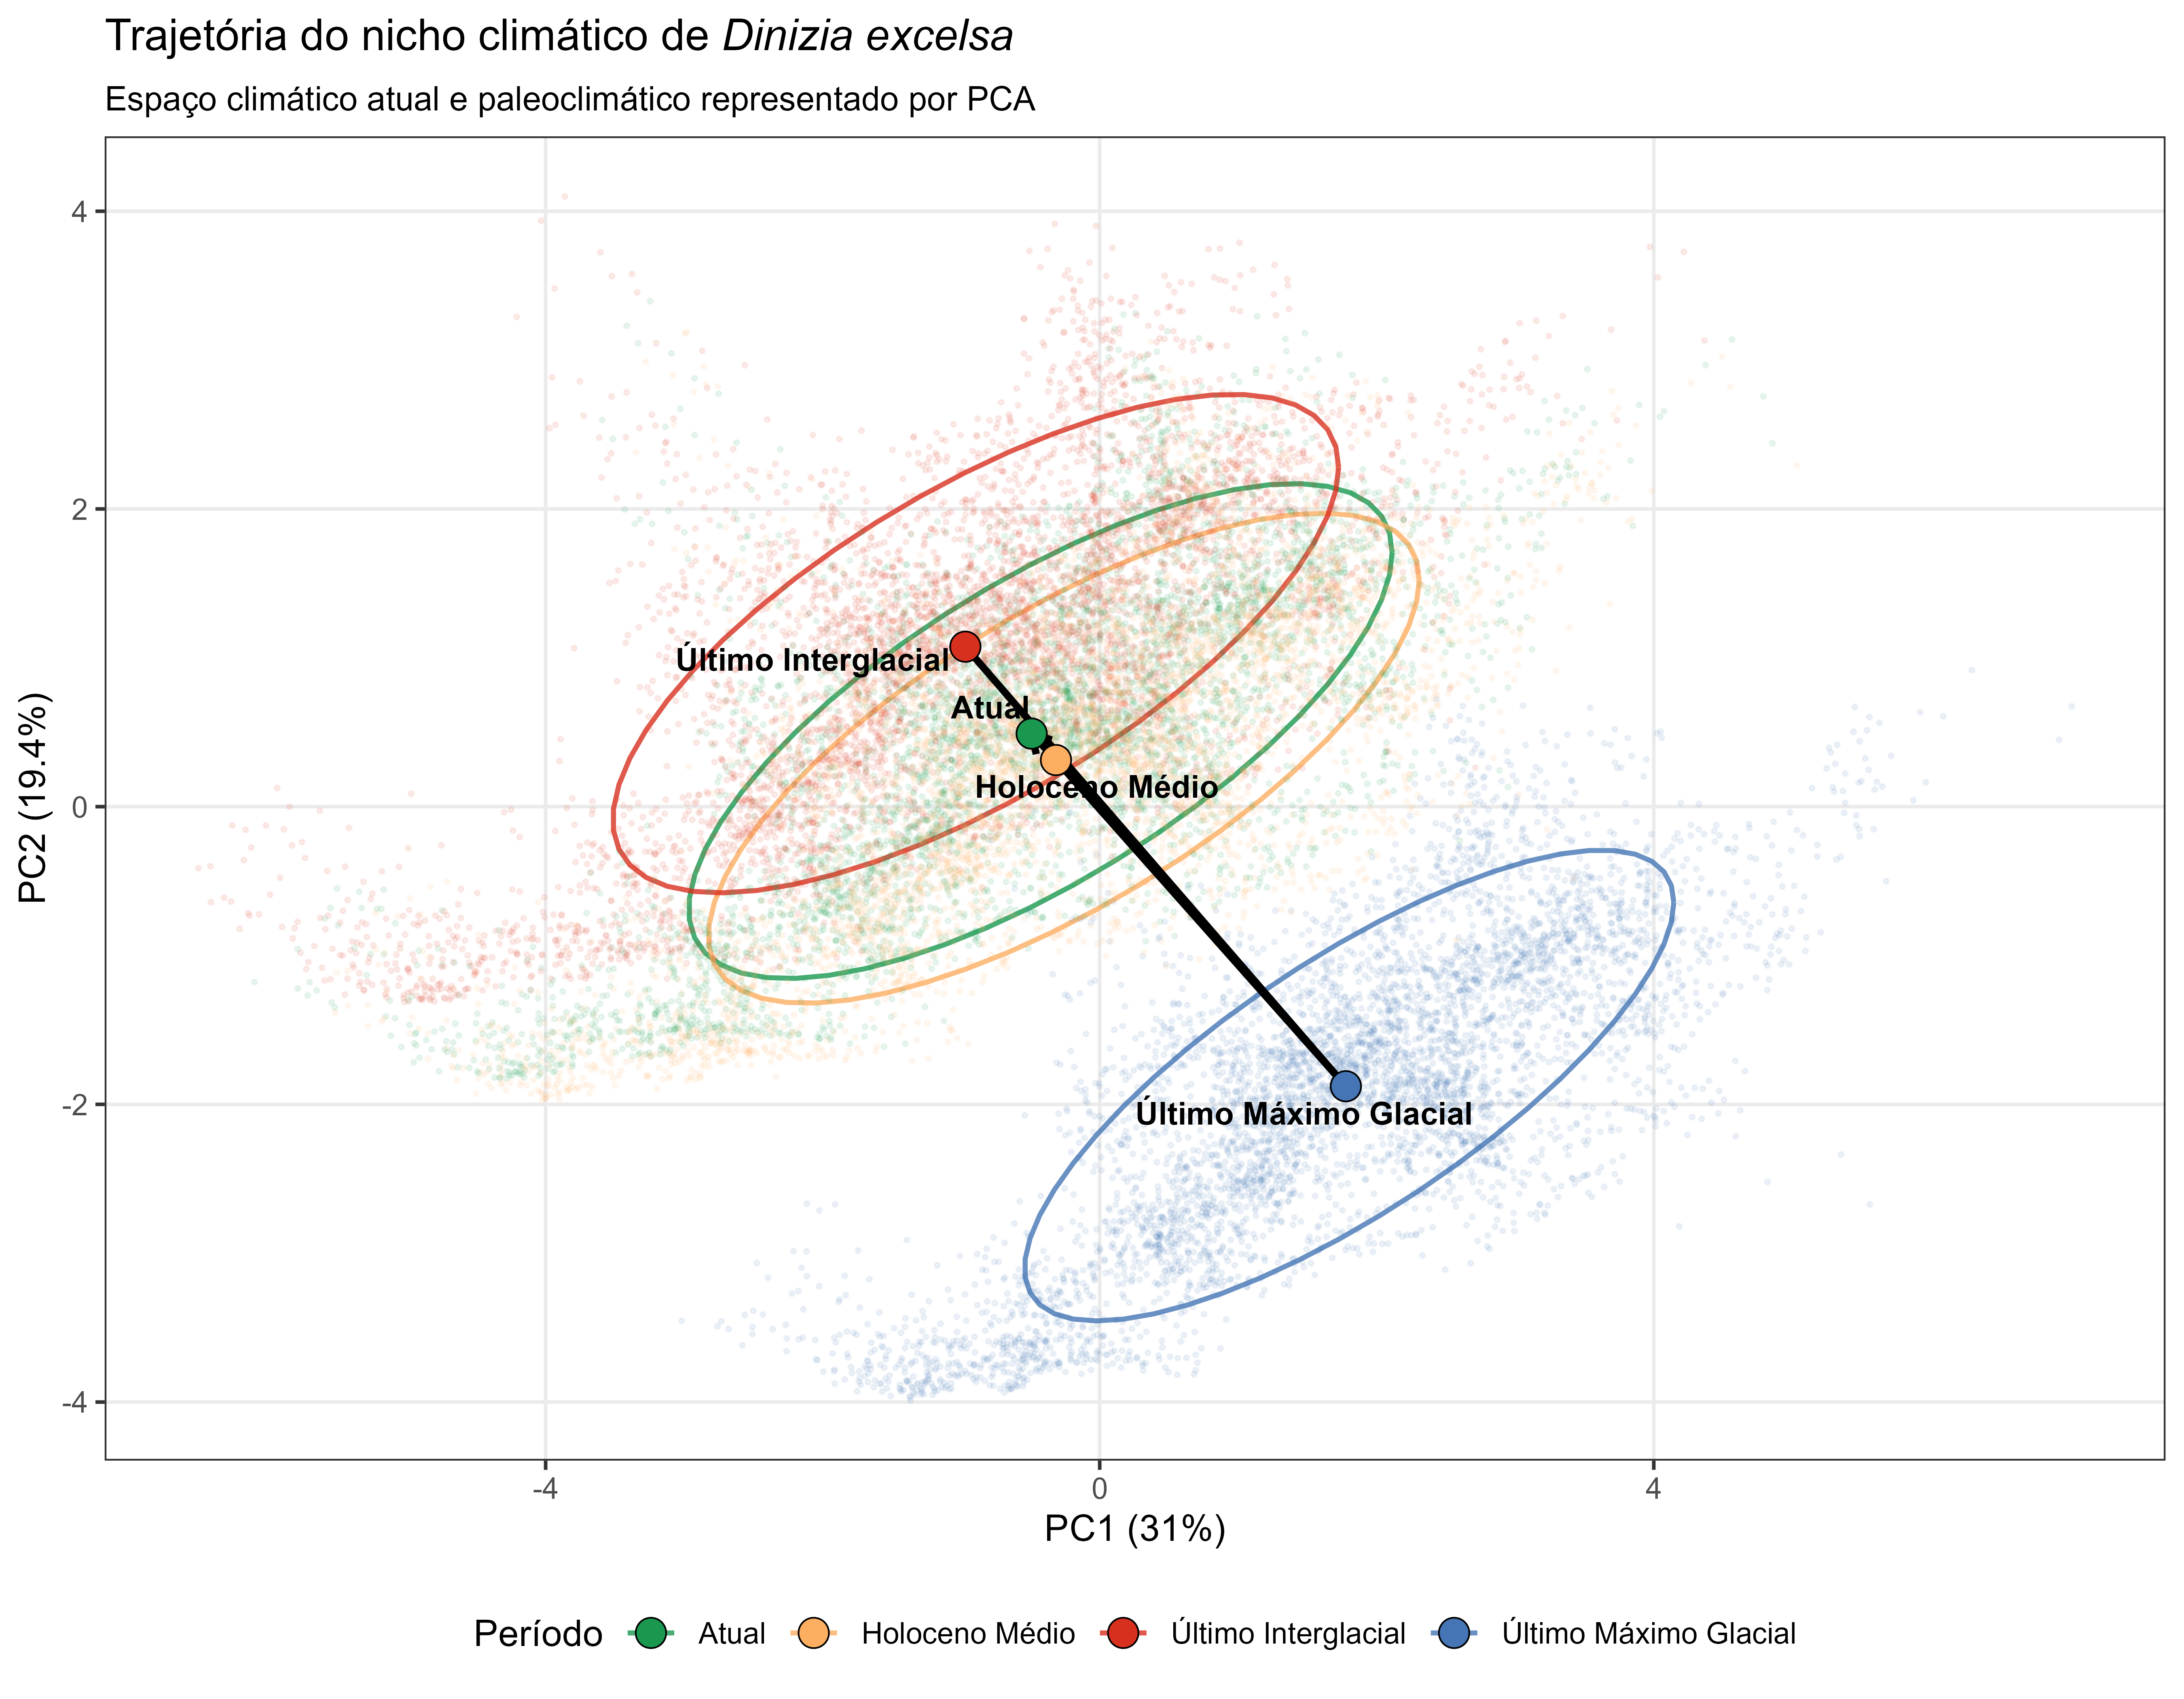
\includegraphics[width=0.88\textwidth]{figuras/unidade15/unidade15_pca_nicho_passado.png}
\caption{Contemporary and paleoclimatic environments for \textit{Dinizia excelsa} represented in a common PCA space.}
\label{fig:unidade15_pca_nicho_passado}
\end{figure}

\section{Historical stability and candidate climatic refugia}

Areas classified as suitable in the baseline and multiple past periods can be interpreted as candidates for long-term climatic stability. They do not prove the existence of refugia or continuous occupation. Threshold choice, temporal resolution, GCM disagreement, sea-level and land-cover changes, dispersal history, and environmental extrapolation all affect the inferred pattern.

\rscriptfile{scripts/unidade15/06_estabilidade_refugios_paleoclimaticos.R}

\begin{figure}[H]
\centering
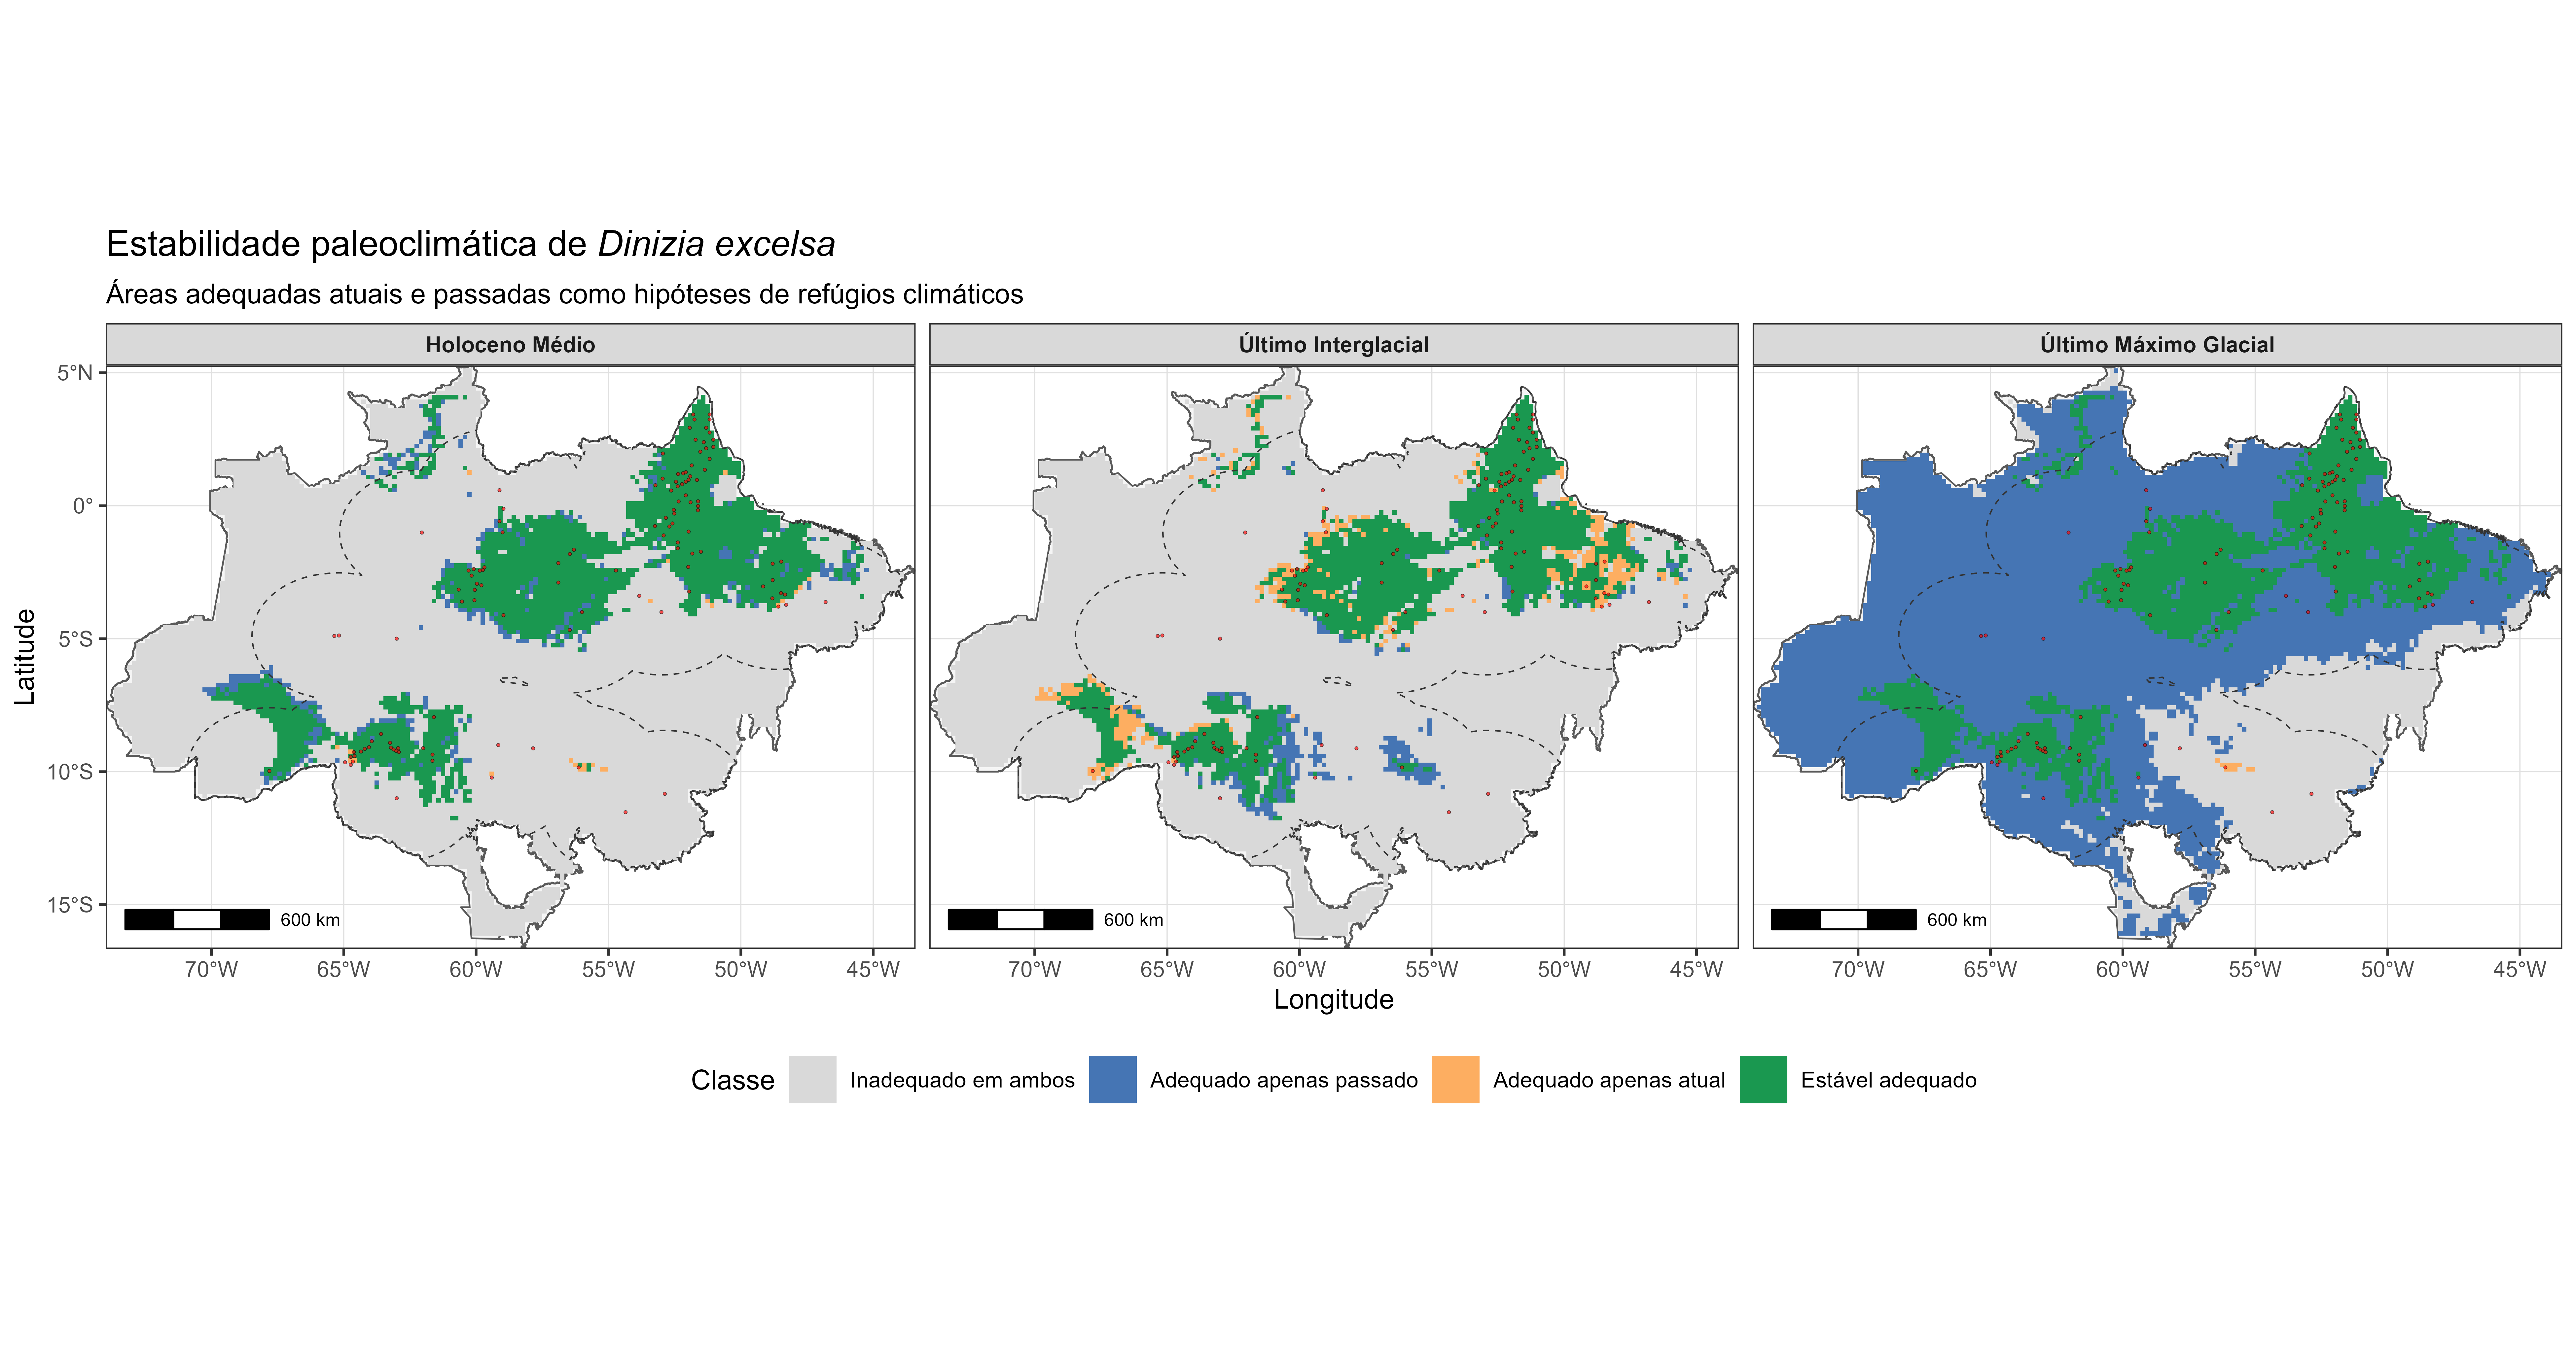
\includegraphics[width=0.96\textwidth]{figuras/unidade15/unidade15_estabilidade_refugios.png}
\caption{Modeled paleoclimatic stability and candidate areas of long-term climatic suitability for \textit{Dinizia excelsa}.}
\label{fig:unidade15_refugios}
\end{figure}

\section{Paleoclimatic synthesis}

\rscriptfile{scripts/unidade15/07_sintese_paleoclimatica.R}

\begin{figure}[H]
\centering
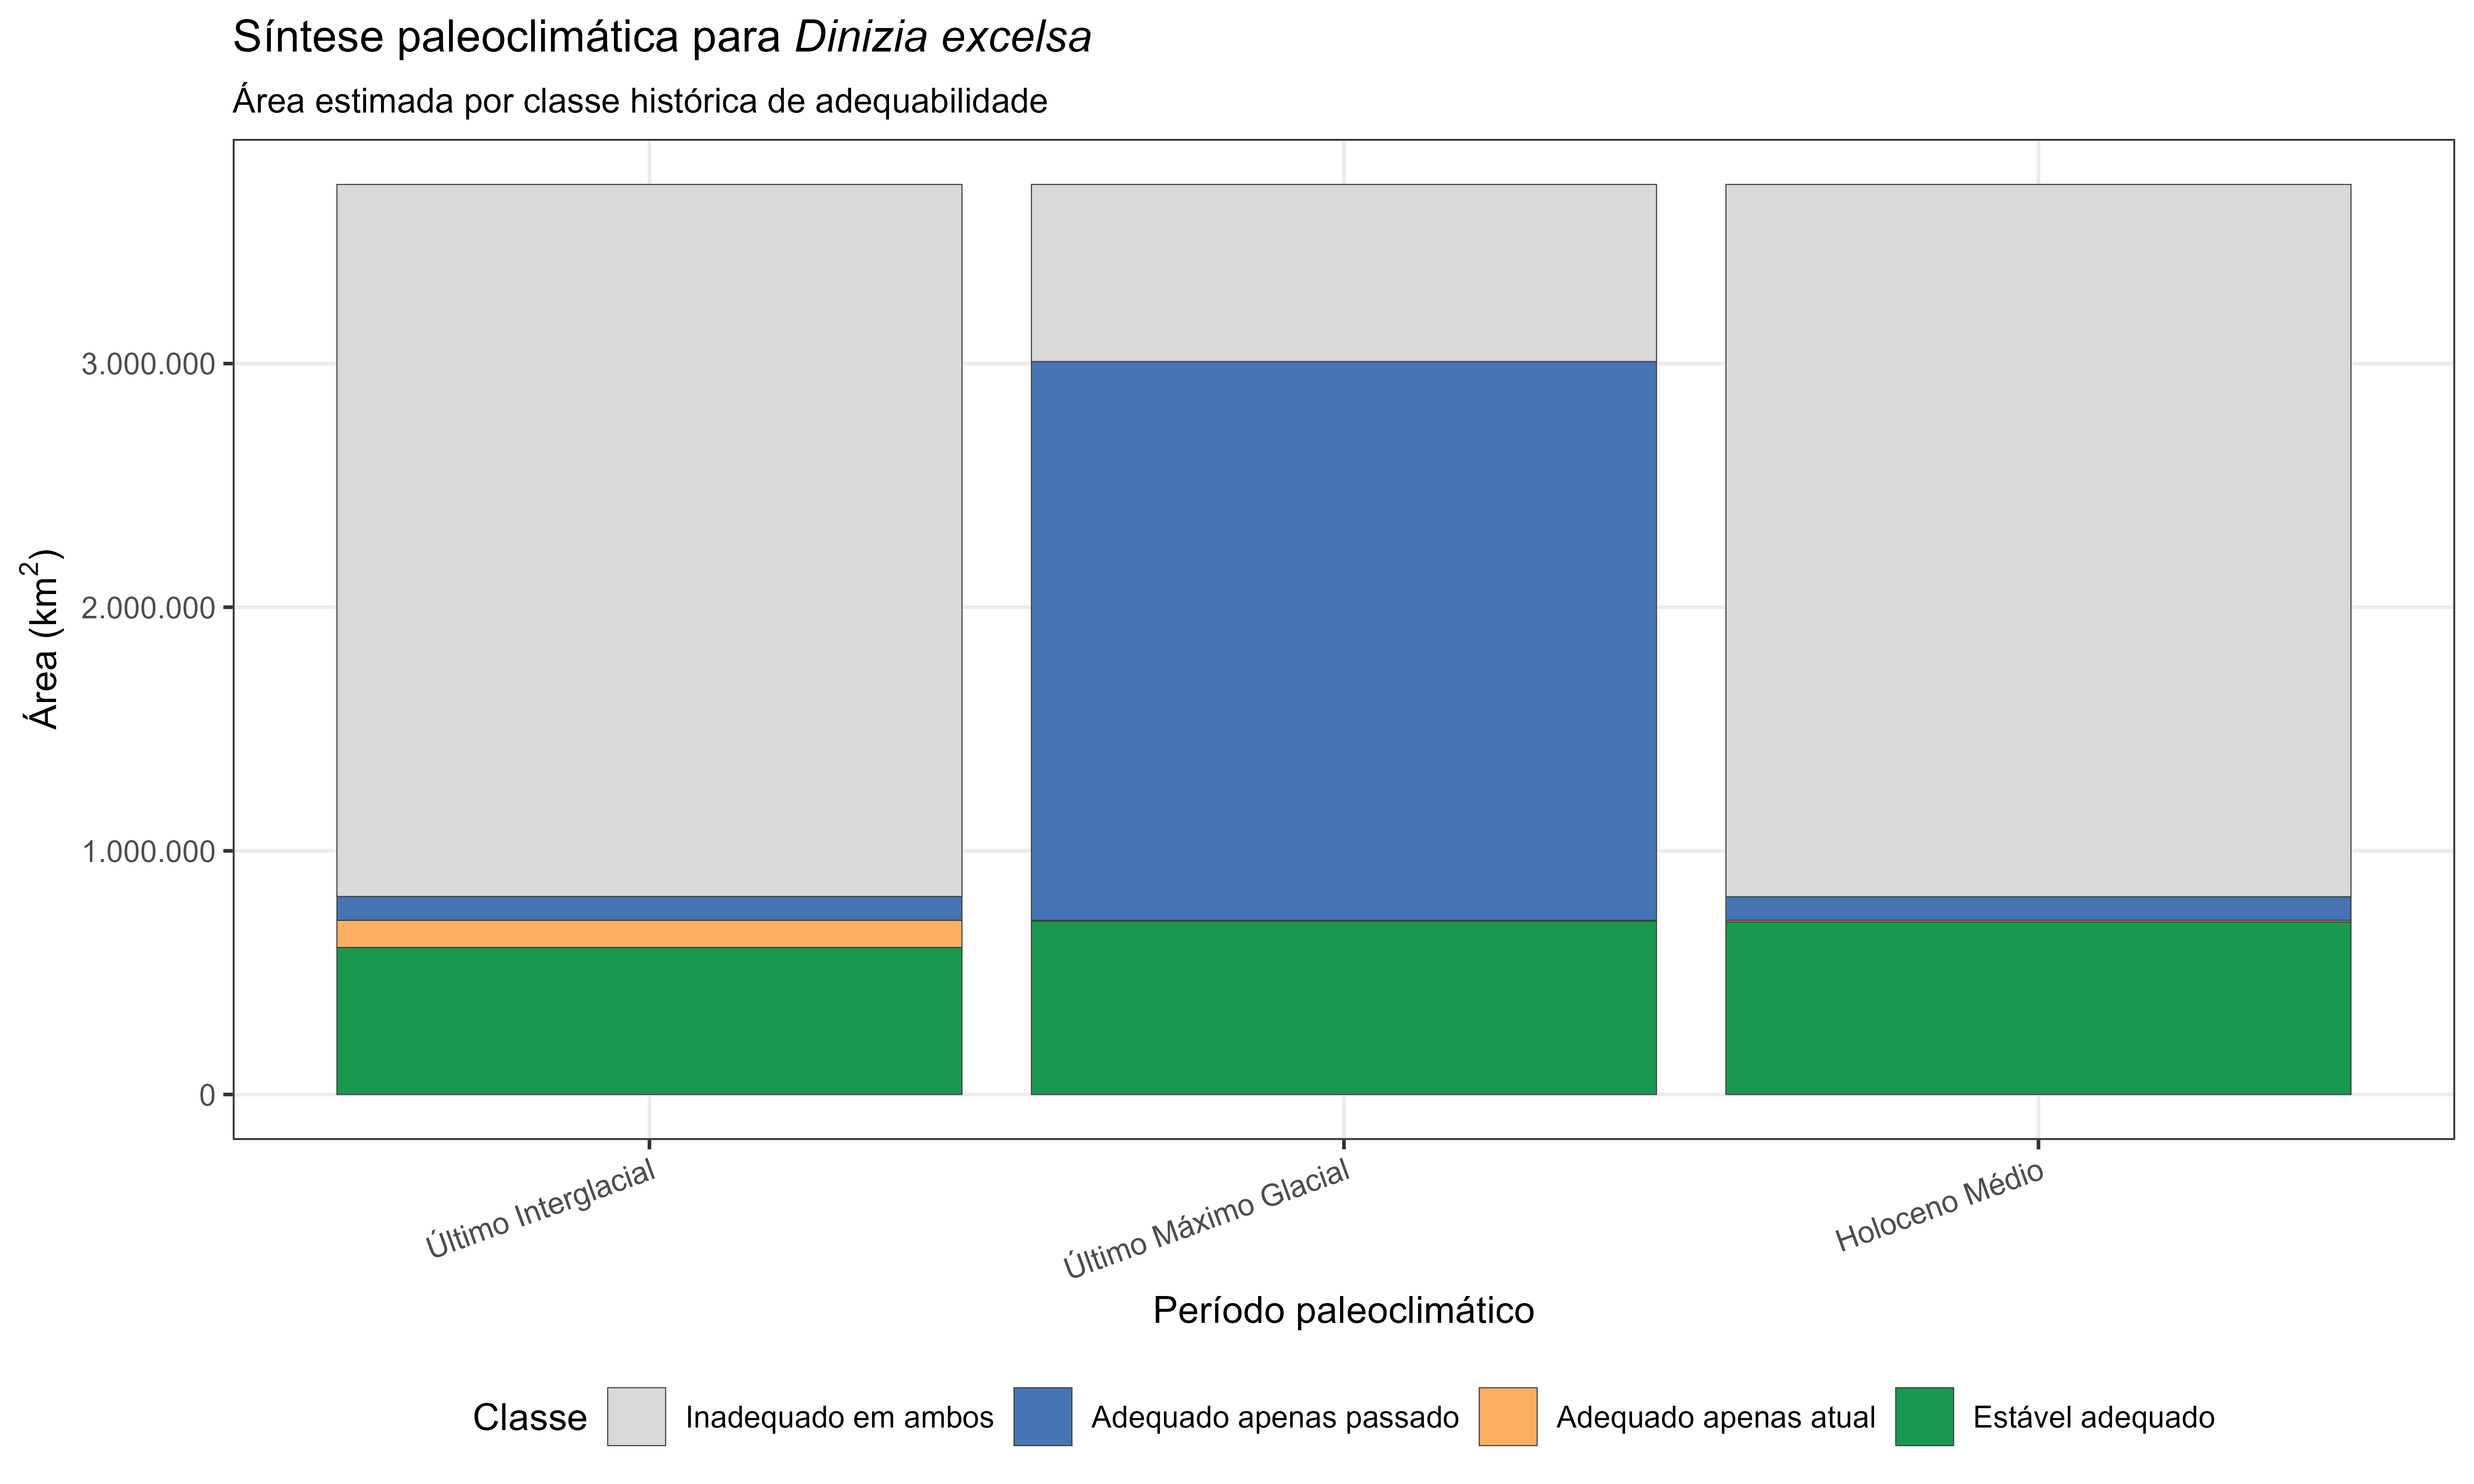
\includegraphics[width=0.88\textwidth]{figuras/unidade15/unidade15_sintese_paleoclimatica.png}
\caption{Estimated suitable area for \textit{Dinizia excelsa} across paleoclimatic periods.}
\label{fig:unidade15_sintese}
\end{figure}

\section{Complete pipeline}

\rscriptfile{scripts/unidade15/08_pipeline_paleoclima.R}

\section{Chapter synthesis}

Paleoclimate reconstruction broadens distribution modeling by connecting contemporary climatic associations with environmental history. For \textit{Dinizia excelsa}, it supports hypotheses about climatic stability, possible areas of historical persistence, and the biogeographic processes underlying its present Amazonian distribution. Strong claims about refugia or past occupancy require independent lines of evidence.

\begin{conceito}[title={\faBook\quad Key message}]
Paleoclimate projections indicate where reconstructed past climates may have been compatible with a species' modeled contemporary climatic association. They do not establish where the species actually occurred.
\end{conceito}

\section{Review exercises}

\begin{enumerate}
\item Distinguish baseline climate, future climate projections, and paleoclimate reconstructions in SDM.
\item What assumptions are made when a contemporary model is projected to the Last Glacial Maximum?
\item Why are temporally stable cells only candidates for climatic refugia?
\item What are the principal sources of uncertainty in paleoclimate SDM projections?
\item How should a common PCA be constructed to compare climatic space across periods?
\item Why is niche conservatism an important, testable assumption in this analysis?
\item Which independent evidence could be combined with paleoclimate projections to inform conservation of Amazonian species?
\end{enumerate}

